\chapterimage{golden_gate.jpg}

\chapter{Layer 3: Internet(work) communication}\label{sec:layer3}

\begin{minipage}{0.4\linewidth}
\begin{center}
\begin{bytefield}{16}
\bitbox{16}{Layer 7: Application} \\
\bitbox{16}{Layer 4: Transport} \\
\bitbox{16}{\color{color1} Layer 3: Internet} \\
\bitbox{16}{Layer 2: Network (LAN)} \\
\bitbox{16}{Layer 1: Physical} \\
\end{bytefield}
\end{center}
\end{minipage}
\begin{minipage}{0.6\linewidth}
\begin{center}
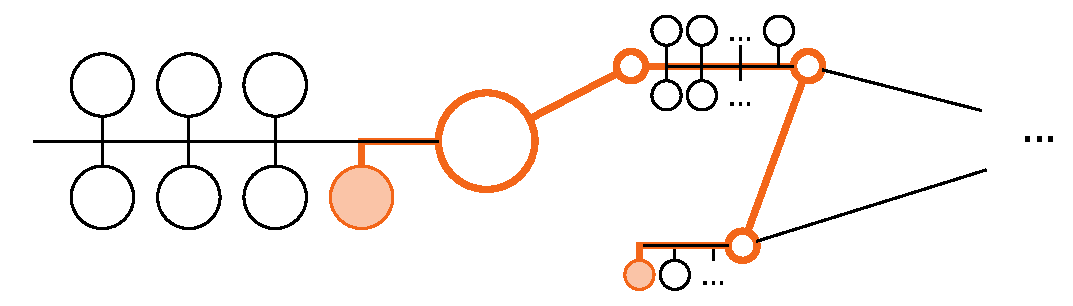
\includegraphics[width=\linewidth]{network_layer3.pdf}
\end{center}
\end{minipage}

\vspace{-0.75cm}

\subsection*{Capabilities}

The \conceptRef{IP}{Internet Protocol (IP)} allows exchanging \concept{datagrams} 
(Layer~3 \conceptRef{PDU}{PDUs}) between devices from different \conceptRef{LAN}{LANs}.
% 
Its addressing system identifies devices globally and makes it possible to 
\conceptRef{routing}{route} datagrams anywhere we need. 

Devices communicating via IP may belong to LANs
based on different technologies and with different types of \concept{MAC} address.
This has two implications:
\begin{itemize}
  \item A datagram that ``fits'' in the \concept{MTU} of the source LAN
    may be too large for the destination's (or any intermediate's) LAN MTU. 
    IP defines a \concept{fragmentation} system to split datagrams,
    which are reconstructed only at the final destination.\\[-0.25cm]
    
  \item When we send a datagram, we know the target device's \conceptRef{IP}{IP address},
  but not necessarily its \concept{MAC} address. Only if we are part of the destination
  LAN we will need that MAC. IP uses \concept{ARP} to translate known IP addresses
  to MAC addresses of the destination LAN's type.

\end{itemize}



\conceptRef{datagram}{Datagrams} may travel through networks not controlled 
by neither the source nor the destination, so datagrams may be lost, reordered and duplicated.
% 
Layer~3 does not provide mechanisms to deal with this; upper layers must implement
protection mechanisms when required 
(\eg, to implement \concept{TCP}'s \conceptRef{stream}{data streams}).


\vspace{-0.25cm}
\subsection*{Protocols}

Version~4 of \concept{IP} is \textit{the} protocol used in Layer~3, \ie,
it is common to virtually all communications in the Internet as we know it today.
% 
For many years, the Internet has been struggling to transition towards \concept{IPv6}, 
but the process is not complex and only \concept{IPv4} provides global coverage.

\concept{IPv4} delegates in the \concept{ARP} protocol the translation of known IP addresses 
into MAC addresses within each LAN. ARP does \textit{not} use IP datagrams.

The following protocols encapsulate their \conceptRef{PDU}{PDUs} in the payload of IP 
\conceptRef{datagram}{datagrams}:\\[-0.6cm]
\begin{itemize}
\item Transport Control Protocol (\concept{TCP}) 
\item User Datagram Protocol (\concept{UDP})
\item Internet Control Message Protocol (\concept{ICMP})
\end{itemize}


\subsection*{Addressing}

\concept{IPv4} addresses are $32$~bit long. They are most often presented to humans in
the \concept{quad decimal} format, \eg, \otherBase{142.250.201.67}. 

Most IP addresses are \conceptRef{public IP}{public} and unique across the Internet, 
\ie, the previous IP has the same meaning worldwide: it identifies a single connected device.

Many addresses are (\conceptRef{reserved IP address}{reserved/private}) and can only be 
used within a particular scope, \eg, a LAN. 
Some of the most common are the following (there are some more):

\begin{center}
\begin{tabular}{ll}
\toprule
\textbf{IP address block} & \textbf{Address scope} \\
\toprule
\otherBase{127.*.*.*} & Computer \\
\otherBase{169.254.*.*} & Local connection (\eg ppp) \\
\otherBase{10.*.*.*} & This LAN \\
\otherBase{172.16.*.*} & This LAN \\
\otherBase{192.168.*.*} & This LAN \\
\otherBase{255.255.255.255} & Limited (IP) broadcast \\
\bottomrule
\end{tabular}
\end{center}

\subsection*{Practical aspects}

The \inlineCode{ip address}, \inlineCode{ip route} and \inlineCode{ip neighbor} commands 
(among others) let you query several aspects of your IP configuration.

\begin{exercise}\ \\[-0.5cm]
\begin{itemize}
\item How many different \concept{IPv4} addresses are there (including reserved and private)? 
\item Are they sufficient now and in the future?
\item Is it problematic that an address like \otherBase{192.168.0.1} can be used by thousands
  of computers in the Internet right now?
\end{itemize}
\end{exercise}


\section{IP -- Internet Protocol}

\subsection*{Packet format}

\concept{IP} defines a \concept{packet} format with a \concept{header} 
that is \textit{at least} $20$~bytes long. Optional parts may be included,
as long as the total header size is a multiple of $32$~bits ($4$~bytes).
The payload can be empty, so the minimum datagram size is $20$~bytes.\\

\begin{center}
\small
\begin{bytefield}[bitheight=3em]{32}
\bitheader{0-31}\\
\begin{rightwordgroup}[curlyshrinkage=10pt]{Mandatory Header ($20$~bytes)}
  \bitbox{4}{IP\\Version} 
  & \bitbox{4}{IHL\\{\scriptsize(HLen/$4$)}} 
  & \bitbox{8}[bgcolor=lightgray]{Type of Service}
  & \bitbox{16}{Datagram Length\\{\scriptsize(Head + Payload, bytes)}} \\
  % 
  \bitbox{16}{Fragment ID} & \bitbox{1}{\otherBase{0}}
  & \bitbox{1}{\rotatebox{90}{\scriptsize DF flag}}
  & \bitbox{1}{\rotatebox{90}{\scriptsize MF flag}}
  & \bitbox{13}{Fragment Offset} \\
  % 
  \bitbox{8}{Time to Live\\(TTL)}
  & \bitbox{8}{Payload protocol}
  & \bitbox{16}[bgcolor=lightgray]{IP Header Checksum}\\
  % 
  \bitbox{32}{Source IP Address} \\
  \bitbox{32}{Destination IP Address}
\end{rightwordgroup} \\
%   
\begin{rightwordgroup}[curlyshrinkage=10pt]{Optional Header (32$\cdot x$ bits)}
\bitbox[tlr]{32}[bgcolor=lightgray]{Options\\{\scriptsize(variable length, optional)}} \\
\bitbox[lbr]{24}[bgcolor=lightgray]{} &
\bitbox{8}[bgcolor=lightgray]{Padding to\\$32$ bits}
\end{rightwordgroup} \\
% 
\begin{rightwordgroup}[curlyshrinkage=10pt]{Payload (8$\cdot y$ bits)}
\bitbox[tlr]{32}{Payload data} \\
\bitbox[lbr]{8}{} & \bitbox[t]{24}{} 
\end{rightwordgroup}
\end{bytefield}
\end{center}

\begin{exercise} \ \\[-0.5cm]
\begin{itemize}
\item How can the payload length be calculated from the header?
\item What is the maximum payload length?
\item What are the possible values of the flags in the IP header?
\item What's longer, an IP address or an Ethernet MAC address?
\item Is it possible to send exactly 17 bits of payload data in an IP datagram?
\item How can we know whether a datagram is encapsulating TCP or UDP data?
\item Why must the optional header part by a multiple of $32$~bits?
\end{itemize}
\end{exercise}

\subsection*{Operation}

When a device A wants to send an IP datagram to a device B, the source and 
destination IPs in the header are fixed and don't change for this datagram.

If devices A and B belong to the same LAN, the datagram is sent directly
(\eg, encapsulated in an Ethernet frame). However, IP can go much farther.
Consider the following scenario, where A wants to communicate with D.

\begin{center}
 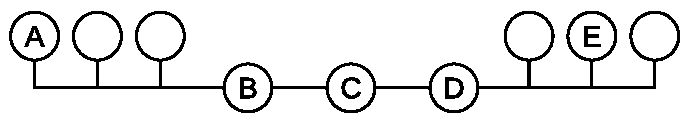
\includegraphics[width=0.5\linewidth]{ip_operation_example.pdf}
\end{center}


Here, the source and destination devices belong to different LANs.
The datagram is passed first to the source's \concept{gateway} router. 
Then, each router passes it to the next one until the datagram reaches 
a router connected to the destination LAN. Finally, that last router 
passes the datagram to the destination. 

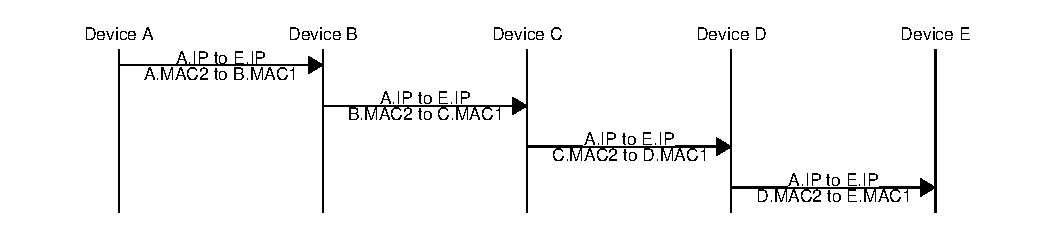
\includegraphics{ip_operation.eps}

\begin{remark}
The source and destination IP addresses don't change throughout the journey.
However, the MAC addresses must correspond to the actual packet transmission within the LAN.
\end{remark}


% \subsection{IP addresses, netmasks and CIDR format}\label{sec:layer3:cidr}
% also division
% 
% \subsection{Fragmentation}
% 
% \subsection{Routing}

\section{ARP -- Address Resolution Protocol}
\begin{remark}
The \concept{ARP} protocol does \textit{not} use IP headers.
\end{remark}

\section{ICMP -- Internet Control Message Protocol}


% - talk about the problem of having different networks, different technologoies (ARPA, XEROX
% - longest prefix matching for routing tables
% - first draft: 8-bit network addresses (a bit off!)
